%
% Acta Acustica united with Acustica -- Instructions for Authors, 2017-03-01
%
\documentclass[twocolumn]{article}

%%%%%%%%%%%%%%%%%%%%%%%%%%%%%%%%%%%%%%%%%%%%%%%
%% Comment / uncomment for one or two column(s) fomat
%\documentclass{article}

\usepackage[modulo,switch]{lineno}
\modulolinenumbers[1]
%%%%%%%%%%%%%%%%%%%%%%%%%%%%%%%%%%%%%%%%%%%%%%%
%% Comment / uncomment for showing line numbers
 \linenumbers

\usepackage[utf8]{inputenc}
\usepackage{amsmath}
\usepackage{amssymb}
\usepackage{float}
\usepackage{graphicx}
\usepackage{algorithm}
\usepackage[noend]{algpseudocode}
\usepackage{caption}
\usepackage{subcaption}

\makeatletter\@ifundefined{date}{}{\date{}}
\makeatother

%\markright{\hfill Kergomard {\em et al.}, p.\ }
\pagestyle{myheadings}

\paperheight297mm \paperwidth210mm
\textwidth170mm  \textheight245mm  \oddsidemargin 20mm
\evensidemargin\oddsidemargin \hoffset-22.4mm \voffset-28.4mm
\topmargin0pt \headheight20mm \headsep4mm \topskip0mm
\footskip17.5mm \columnsep7mm \arraycolsep2pt \parindent10pt
\renewcommand{\abstractname}{Introduction}

\DeclareMathSymbol{\sminus}{\mathbin}{AMSa}{"39}

\begin{document}

\title{TTT4180 Technical Acoustics - Assignment 7}

\author{Nicholas Bresina, Department of Electronic Systems, NTNU Trondheim, Norway \\
nicholdb@stud.ntnu.no}

\maketitle\thispagestyle{empty}

\begin{abstract}
This assignment in the Technical Acoustics course (TTT4180) revolves around
the transmission-line matrix (TLM) simulation technique used for acoustic waves
and studying a variety of acoustic wave propagation scenarios by simulation.

The report is split into two parts, where the first part contains a 
description of the methods used to implement a TLM simulation in Python.
After that, some results generated with said implementation are presented and discussed.

The second part delves deeper into analysis of wave propagation, specifically the sound pressure
level with respect to distance, surface reflections, and the effect of a noise screen.
This part uses a provided GUI tool called TLMfig that implements TLM in Matlab.

Lastly, the report gives a brief outlook with a discussion of difficulties
encountered during this assignment with some additional final conclusions.
\end{abstract}


\section{Wave Propagation in a 2D Pipe}
To analyze the propagation of a wave in a pipe, a 2D TLM implementation was needed.
Python was chosen, as it provides all of the necessary features in libraries such
as Numpy \cite{NumpyManual} for arrays and linear algebra and Matplotlib \cite{Matplotlib}
for plotting the results.

\subsection{Methods}
\subsubsection{TLM}
The implementation is strongly based on the article provided with the assignment,
that describes TLM \cite{KagawaTLM}.
Nevertheless the most important parts will be described in this section.

The main concept is to replace the continuous space with a grid of so-called nodes,
as shown in Fig. \ref{fig_tlm_mesh}.

\begin{figure}[H]
    \centering
    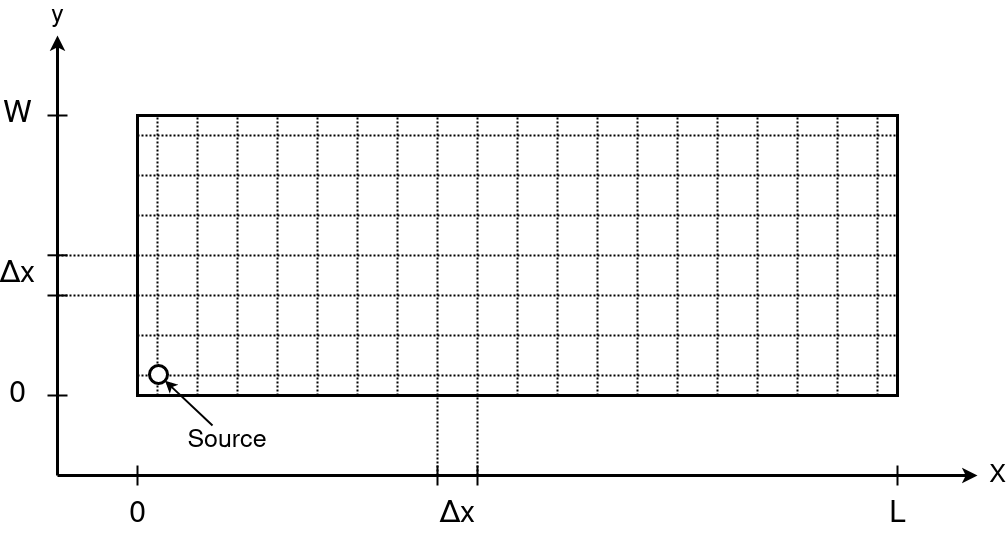
\includegraphics[width=75mm]{./Images/tlm_pipe.png}
    \caption{Example for TLM mesh placed on a pipe with dimensions L$\times$W}
    \label{fig_tlm_mesh}
\end{figure}

Each node can be represented as a pipe system with four branches.
And the nodes will be indexed with $i, j$ referencing their position on the grid.
The branches are modelled as pipes for the propagation of plane waves.
Scattering or outgoing waves are denoted with $_{k}S_{i,j}^{n}$ and incident waves
with $_{k}I_{i,j}^{n}$ respectively.
$k$ is the iteration count and $n$ is the branch index as shown in Fig.
\ref{fig_tlm_node}.

\begin{figure}[H]
    \centering
    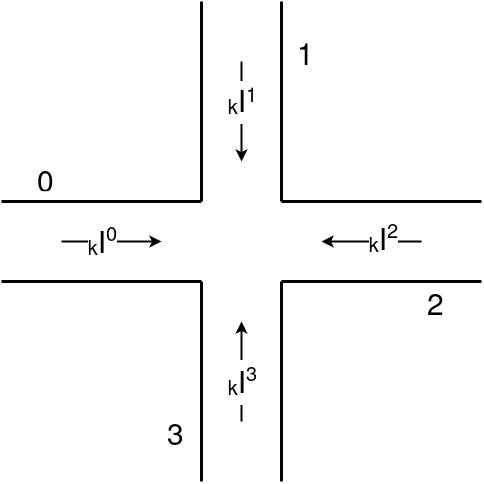
\includegraphics[width=50mm]{./Images/tlm_node_incoming.png}
    \caption{TLM node showing incident and outgoing waves as well as branch indexing}
    \label{fig_tlm_node}
\end{figure}

Due to the impedance discontinuity at the node the incident waves of iteration $k$
will be turned into the scattering waves of iteration $k+1$.

Which can be written as

\begin{equation}
\begin{aligned}
    _{k+1}S_{i,j}^{0} &= \frac{1}{2}\left[\sminus_kI_{i,j}^{0}+_kI_{i,j}^{1}+_kI_{i,j}^{2}+_kI_{i,j}^{3}\right] \\
    _{k+1}S_{i,j}^{1} &= \frac{1}{2}\left[_kI_{i,j}^{0}-_kI_{i,j}^{1}+_kI_{i,j}^{2}+_kI_{i,j}^{3}\right] \\
    _{k+1}S_{i,j}^{2} &= \frac{1}{2}\left[_kI_{i,j}^{0}+_kI_{i,j}^{1}-_kI_{i,j}^{2}+_kI_{i,j}^{3}\right] \\
    _{k+1}S_{i,j}^{3} &= \frac{1}{2}\left[_kI_{i,j}^{0}+_kI_{i,j}^{1}+_kI_{i,j}^{2}-_kI_{i,j}^{3}\right] \\
\end{aligned}
\end{equation}

This can then be rewritten using the \textit{scattering matrix} as follows

\begin{equation}
\begin{bmatrix}
    _{k+1}S_{i,j}^{0} \\
    _{k+1}S_{i,j}^{1} \\
    _{k+1}S_{i,j}^{2} \\
    _{k+1}S_{i,j}^{3} \\
\end{bmatrix}
=
\frac{1}{2}
\begin{bmatrix}
    \sminus1 & 1 & 1 & 1 \\
    1 & \sminus1 & 1 & 1 \\
    1 & 1 & \sminus1 & 1 \\
    1 & 1 & 1 & \sminus1 \\
\end{bmatrix}
\begin{bmatrix}
    _kI_{i,j}^{0} \\
    _kI_{i,j}^{1} \\
    _kI_{i,j}^{2} \\
    _kI_{i,j}^{3} \\
\end{bmatrix}
\label{eq_scattering_matrix}
\end{equation}

The factor $\frac{1}{2}$ is due to the fact that the energy is split evenly to four branches.
Resulting in a factor of $\frac{1}{4}$ with respect to the energy.
Due to $W \propto p^{2}$ we can establish a factor of $\frac{1}{2}$ for the
pressure magnitude.

The incident waves of the next iteration are related to the scattering waves generated by the
incident waves of the current iteration.
The scattering waves propagate to the branches of the neighboring nodes, which is shown in
Fig. \ref{fig_tlm_nodes_transmission}.

\begin{figure}[H]
    \centering
    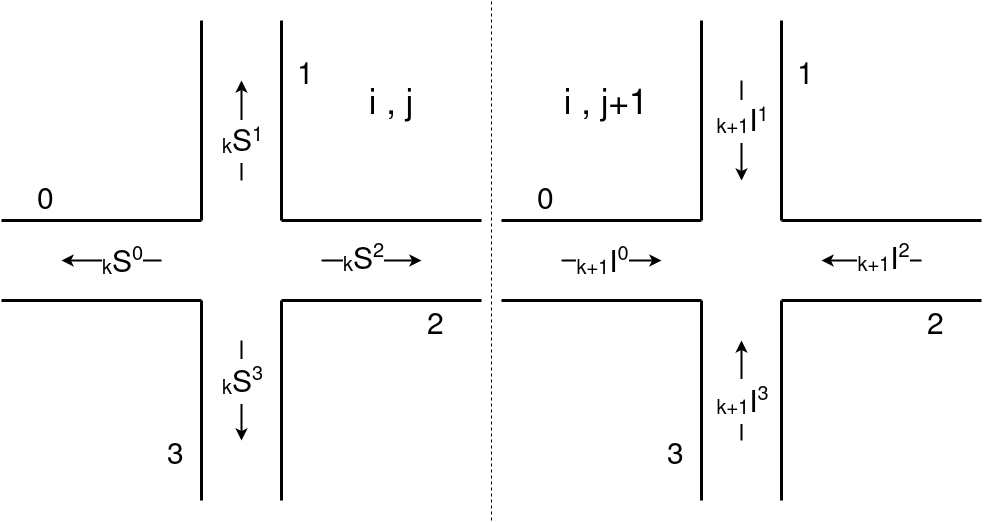
\includegraphics[width=75mm]{./Images/tlm_nodes_transmission.png}
    \caption{TLM nodes depicting the propagation of the scattering wave of branch $2$ to the incident wave of branch $0$ for the next iteration}
    \label{fig_tlm_nodes_transmission}
\end{figure}

Mathematically this can be written with the following equations

\begin{equation}
\begin{aligned}
    _{k+1}I_{i,j}^{0} &= _{k}S_{i,j\sminus 1}^{2} \\
    _{k+1}I_{i,j}^{1} &= _{k}S_{i,j\sminus 1}^{3} \\
    _{k+1}I_{i,j}^{2} &= _{k}S_{i,j+1}^{0} \\
    _{k+1}I_{i,j}^{3} &= _{k}S_{i,j+1}^{1} \\
\end{aligned}
\label{eq_propagation}
\end{equation}

These relations only count for all the nodes, that are not part of any of the boundaries.
At the boundary the next iteration's incident wave is given by the branch's
scattering wave and the boundary's reflection coefficient $R_{m}$.

\begin{equation}
    _{k+1}I_{i,j}^{n} = R_{m}\cdot _{k}S_{i,j}^{n}
    \label{eq_boundary_propagation}
\end{equation}

The pressure can be calculated by the superposition of all the incident waves in the node,
as given with

\begin{equation}
    _{k}p_{i,j} = \sum_{i=0}^{3} {}_kI_{i,j}^{n}
\end{equation}

\subsubsection{Python Implementation}
In the Python code the nodes are represented as an array.
Where the size of the array is given by the physical dimensions L$\times$W and
the requirement to $\Delta x$, shown in Fig. \ref{fig_tlm_mesh}, which is

\begin{equation}
    \Delta x \leq \frac{\lambda_{max}}{10}
    \label{eq_delta_x}
\end{equation}

Where $\lambda_{max}$ is the wavelength of the maximum frequency that should be possible
to represented in the model, which is given by

\begin{equation}
    \lambda_{max} = \frac{c}{f_{max}}
    \label{eq_max_wavelength}
\end{equation}


The size of the arrays $M\times N$ is then calculated by
\begin{equation}
\begin{aligned}
    M &= ceil\left(\frac{\text{L}}{\Delta x}\right) \\
    N &= ceil\left(\frac{\text{W}}{\Delta x}\right) \\
\end{aligned}
\label{eq_integer_dimension}
\end{equation}

Because a wave propagates the distance $\Delta x$ in one iteration of the simulation,
this also gives the timestep with

\begin{equation}
    \Delta t = \frac{\Delta x}{c}
    \label{eq_delta_t}
\end{equation}

The easiest way to represent the different branches and differentiate between incident
and scattering wave is by using a multidimensional array.
The first two dimensions are the spatial integer dimensions $M\times N$.
The third dimension is used to stack one grid for each branch waves, as shown in Fig. \ref{fig_python_layers}.
So the resulting array has the shape $\left(M, N, 4\right)$.
An additional layer is used to store source amplitudes on the grid, which are written as $_{k}G_{i,j}$.

\begin{figure}[H]
    \centering
    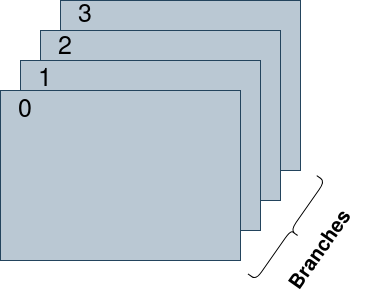
\includegraphics[width=60mm]{./Images/python_layers.png}
    \caption{Depiction of the layers used in the implementation}
    \label{fig_python_layers}
\end{figure}

To have efficient computation two of these multidimensional arrays are being used,
where one corresponds to the current step and the other to the next iteration.
With that, the values can easily be updated without generating temporary objects.
The full shape of the array is then given with $\left(M, N, 9, 2\right)$.

Eq. \ref{eq_scattering_matrix} has to be rewritten to allow incorporating the
mentioned source layer.

\begin{equation}
\begin{bmatrix}
    _{k+1}S_{i,j}^{0} \\
    _{k+1}S_{i,j}^{1} \\
    _{k+1}S_{i,j}^{2} \\
    _{k+1}S_{i,j}^{3} \\
\end{bmatrix}
=
\frac{1}{2}
\begin{bmatrix}
    \sminus1 & 1 & 1 & 1 & 1\\
    1 & \sminus1 & 1 & 1 & 1\\
    1 & 1 & \sminus1 & 1 & 1\\
    1 & 1 & 1 & \sminus1 & 1\\
\end{bmatrix}
\begin{bmatrix}
    _kI_{i,j}^{0} \\
    _kI_{i,j}^{1} \\
    _kI_{i,j}^{2} \\
    _kI_{i,j}^{3} \\
    _{k+1}G_{i,j} \\
\end{bmatrix}
\label{eq_source_scattering_matrix}
\end{equation}

Which will add the sources' amplitudes to the corresponding scattering wave values.

Updating the incident waves can be done just as described in the TLM chapter.

To update the nodes' values for one iteration the following steps are needed:
\begin{algorithm}[H]
\caption{Update steps for one iteration}
\begin{algorithmic}[1]
    \Procedure{update\_tlm}{}
    \For{all sources}
        \State update source amplitude
    \EndFor
    \For{m \textbf{in} M}
        \For{n \textbf{in} N}
            \State compute current scattering wave values
        \EndFor
    \EndFor
    \For{m \textbf{in} M}
        \For{n \textbf{in} N}
            \State update incident waves of next iteration
        \EndFor
    \EndFor
    \State update iteration step count
    \EndProcedure
\end{algorithmic}
\end{algorithm}

\subsection{Calculations}
The pipe dimensions that are used within this assignment are $\text{L}=2\text{m}$
and $\text{W}=0.2\text{m}$.
And the maximum considered frequency is $2 \text{kHz}$.

Given $c=343\text{m/s}$ and using Eqs. (\ref{eq_max_wavelength}), (\ref{eq_delta_x}),
and (\ref{eq_delta_t}) we receive the following values,

\begin{equation}
\begin{aligned}
    \lambda_{max} &= 0.1715\text{m} \\
    \Delta x &= \frac{\lambda_{max}}{10} = 0.01715\text{m} \\
    \Delta t &= 50\mu\text{s} \\
\end{aligned}
\end{equation}

\subsubsection{Modes}
With the assumption that all boundaries are rigid walls we can calculate the modal
frequencies \cite{CavitiesWaveguides} with

\begin{equation}
    f_{lm} = \frac{c}{2}\sqrt{\left(\frac{l}{L}\right)^2 + \left(\frac{m}{W}\right)^2}
\end{equation}

Resulting in the following list of modes:

\begin{center}
\begin{tabular}{c|r}
    ($l$,$m$) & $f_{lm}$ [Hz] \\
    \hline
    (1,0) & 85.75 \\
    (2,0) & 171.50 \\
    (3,0) & 257.25 \\
    (4,0) & 343.00 \\
    (5,0) & 428.75 \\
    (0,1) & 857.50 \\
    (1,1) & 861.78 \\
\end{tabular}
\end{center}

From this we can conlude that there should not be a mode in y-direction below $857.5\text{Hz}$
and only plane waves should be present.

All the modes where $m=0$ can be considered the resonance frequencies of the closed-closed
pipe \cite{PipesResonators}.
Which are given by

\begin{equation}
    kL = \pi l
\end{equation}

\subsection{Results}
\begin{figure}[H]
    \begin{subfigure}[]{75mm}
        \centering
        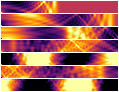
\includegraphics[width=75mm]{./Images/pipe_evolution_r1.png}
        \caption{Right boundary with R $= 1$}
        \label{fig_pipe_evo_r1}
    \end{subfigure}
    \begin{subfigure}[]{75mm}
        \centering
        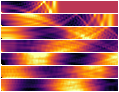
\includegraphics[width=75mm]{./Images/pipe_evolution_r01.png}
        \caption{Right boundary with R $= 0.1$}
        \label{fig_pipe_evo_r01}
    \end{subfigure}
    \caption{Evolution of the wave in the pipe over time}
    \label{fig_pipe_evolution}
\end{figure}

From Fig. \ref{fig_pipe_evolution} we can observe how the wave propagates when a sine wave source
is placed in the bottom left corner with $500 \text{Hz}$.
The first image (Fig. \ref{fig_pipe_evo_r1}) shows the case where the right boundary is a rigid wall.
In that case we can observe that a mode is established with standing nodes.
The wave's minima and maxima flip according to the source's amplitude.

In the case that the right boundary has a reflection coefficient of $0.1$ (Fig. \ref{fig_pipe_evo_r01}
the behavior is slightly different.
Instead of standing nodes, they now move toward the pipe end corresponding to source's excitation.

\section{TLMfig}
\subsection{Propagation in free space}
\subsubsection{Description}
To analyze the behavior of the amplitude of the wave with respect to distance a source and
microphones are placed along one line, as shown in Fig. \ref{fig_3_1_example}.

\begin{figure}[H]
    \centering
    
\includegraphics[width=60mm]{./Images/tlmfig_3_1.png}
    \caption{Simplified example for source and microphone setup to analyze propagation in free space}
    \label{fig_3_1_example}
\end{figure}

In the actual simulation the source was placed in the coordinates $\left(1,50\right)$ and
the 30 microphones where placed at $\left(3n+2,50\right)$, where $n\in\left[0,30\right[$.
The source was configured to produce a sine wave with an amplitude of one and a
number of cells per wavelength (NCPW) of $15$.

\subsubsection{Results}
The signal arrivals at the microphones can be seen in Fig. \ref{fig_3_1_3D}.
The microphones with a higher index are further away.
This is also visible through the delayed arrivals at the start.

\begin{figure}[H]
    \centering
    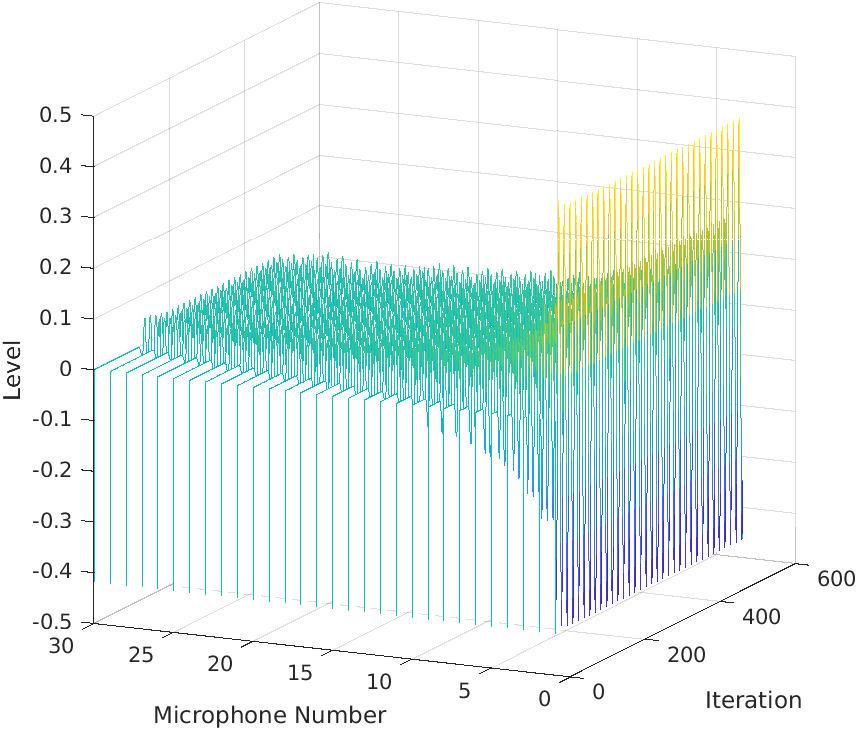
\includegraphics[width=75mm]{./Images/3_1_3d.png}
    \caption{3D graph of the received signals at the microphones}
    \label{fig_3_1_3D}
\end{figure}

With these signals we can calculate the sound pressure levels (SPLs) and plot
them against the distance, which is depicted in Fig. \ref{fig_3_1_spl}.
The calculation was performed by averaging the peak amplitudes and then
referencing against $p_0 = 20\mu\text{Pa}$.

\begin{equation}
    SPL = 20\log_{10}\left(\frac{p_{peak,mean}}{\sqrt{2}\cdot p_{0}}\right)
\end{equation}

In the plot shown in Fig. \ref{fig_3_1_spl} we can roughly see the expected
decay over distance.
% Possibly add fitted 1/r curve to plot

\begin{figure}[H]
    \centering
    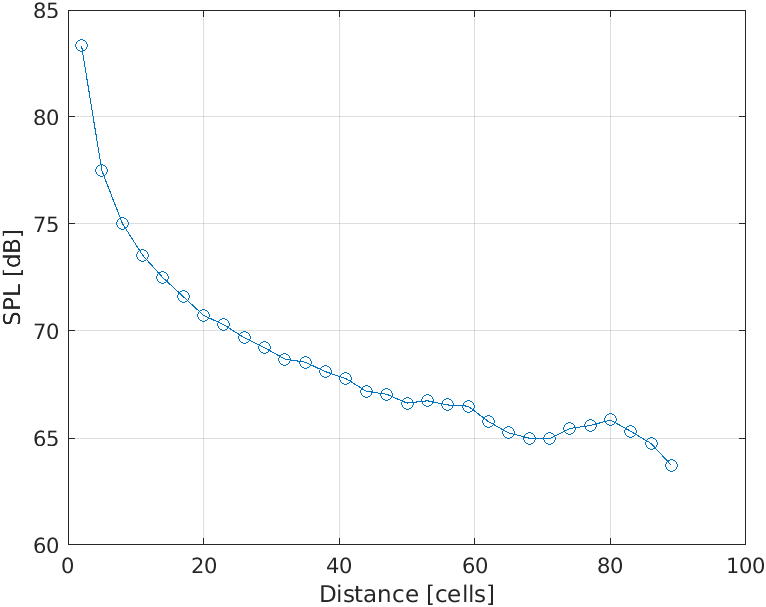
\includegraphics[width=75mm]{./Images/3_1_spls.png}
    \caption{The calculated SPLs for the microphone array against distance}
    \label{fig_3_1_spl}
\end{figure}

\subsection{Reflection from surface}
\subsubsection{Description}
This next simulation is intended to study the behavior of the wave reflected from
surfaces with different reflection coefficient.
For this a surface was placed at the bottom in TLMfig.
The source was placed at $\left(50,59\right)$ and the 20 microphones were
placed at around the same height with the following coordinates
$\left(4n+10,60\right)$, where $n\in\left[0,20\right[$.
The source was set to generate a gaussian pulse with an amplitude of one.

\begin{figure}[H]
    \centering
    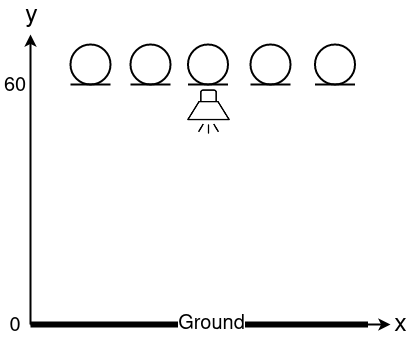
\includegraphics[width=55mm]{./Images/tlmfig_3_2.png}
    \caption{A depiction of the source and microphone arrangement to investigate reflection of surfaces}
    \label{fig_3_2_example}
\end{figure}

\subsubsection{Results}
The signal arrivals are shown in the two plots in Fig. \ref{fig_3_2_3d}.
They show the two received pulses for different reflection coefficients, where
the first pulse is the direct and the second the reflected one.

\begin{figure}[H]
    \begin{subfigure}[]{75mm}
        \centering
        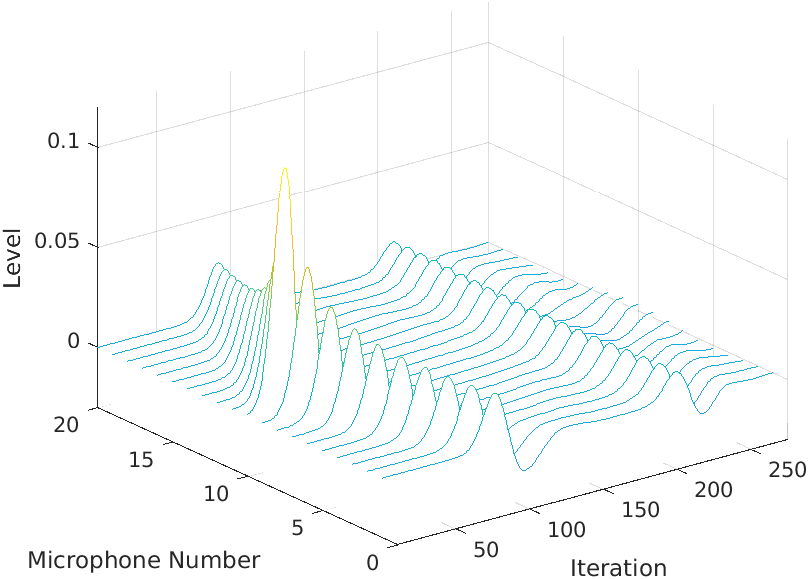
\includegraphics[width=75mm]{./Images/3_2_r_1_3D.png}
        \caption{Reflection coefficient = 1}
        \label{fig_3_2_3d_r_1}
    \end{subfigure}
    \begin{subfigure}[]{75mm}
        \centering
        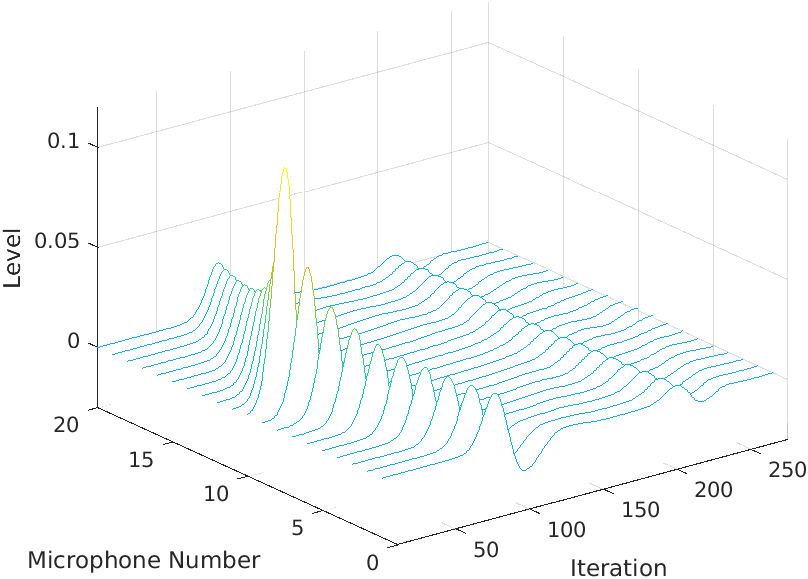
\includegraphics[width=75mm]{./Images/3_2_r_0.5_3D.png}
        \caption{Reflection coefficient = 0.5}
        \label{fig_3_2_3d_r_05}
    \end{subfigure}
    \caption{Signals received at the microphone array with different reflection coefficients}
    \label{fig_3_2_3d}
\end{figure}

Using this data we can plot the loss on the reflected pulse using the direct pulse as a
reference.

\begin{equation}
    \text{Loss} = -20\log_{10}\left(\frac{p_{peak,reflected}}{p_{peak,direct}}\right)
\end{equation}

This is plotted for all the microphones in the array and displayed in Fig. \ref{fig_3_2_plot}.

\begin{figure}[H]
    \centering
    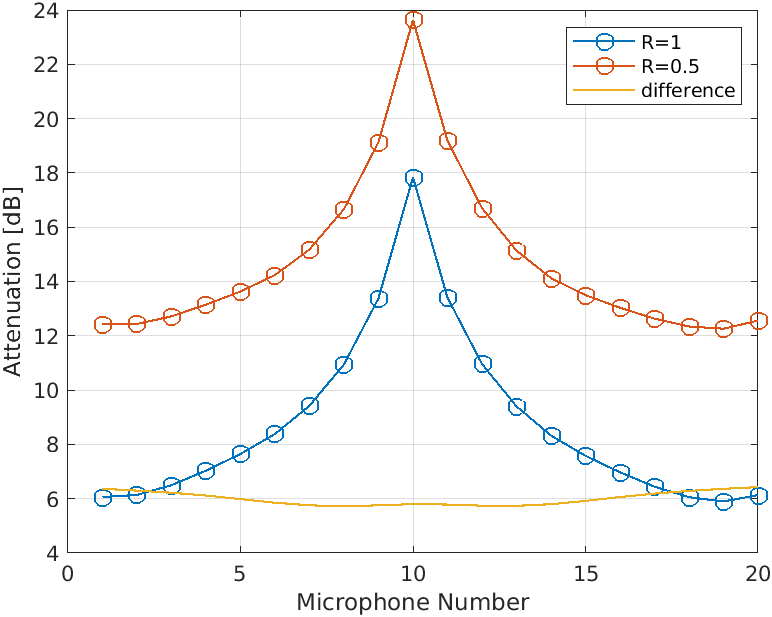
\includegraphics[width=75mm]{./Images/3_2_2D.png}
    \caption{The loss from direct to reflected pulse for the two reflection coefficients}
    \label{fig_3_2_plot}
\end{figure}

It can be observed that halving the reflection coefficient of the surface results in
a loss of $\approx 6\text{dB}$.


\subsection{Effect of noise screen}
\subsubsection{Description}
The last simulation is used to analyze the effect of a noise screen.
In this case the noise screen was simulated as a perfectly rigid wall and
the ground having a reflection coefficient of $0.95$.
The source was setup to produce a sine wave with a NCPW of $15$ and $45$ respectively,
as well as just noise.
Using different NCPW values provides insight in frequency behavior, where a low NCPW
corresponds to higher frequencies.
The simulation arrangement can be seen in Fig. \ref{fig_3_3_example}.

\begin{figure}[H]
    \centering
    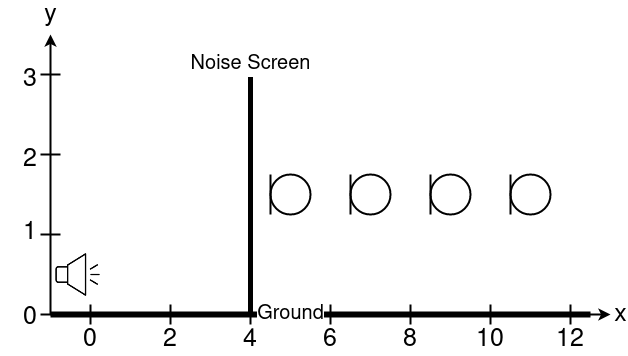
\includegraphics[width=75mm]{./Images/tlmfig_3_3.png}
    \caption{A simplified diagram of source and microphone arrangement for the noise screen simulation}
    \label{fig_3_3_example}
\end{figure}

The exact setup is given by the ground being at height of $10$ cells, the source at $\left(10,12\right)$, the
screen expands from $\left(18,10\right)$ to $\left(18,22\right)$, and the ten microphones have the coordinates
$\left(4n+20,16\right)$ with $n\in\left[0,10\right[$.
To analyze the effect of the screen the simulation is run once with and once without screen.

\subsubsection{Results}
In Fig. \ref{fig_3_3_3d} an example is given where the provided source type was noise.
The data from these two simulations per source can be used to calculate the \textit{insertion loss}.
The loss that results from adding the screen is given by

\begin{equation}
    \text{Insertion Loss} = 20\log_{10}\left(\frac{p_{rms,direct}}{p_{rms,screen}}\right)
\end{equation}

\begin{figure}[H]
    \begin{subfigure}[]{75mm}
        \centering
        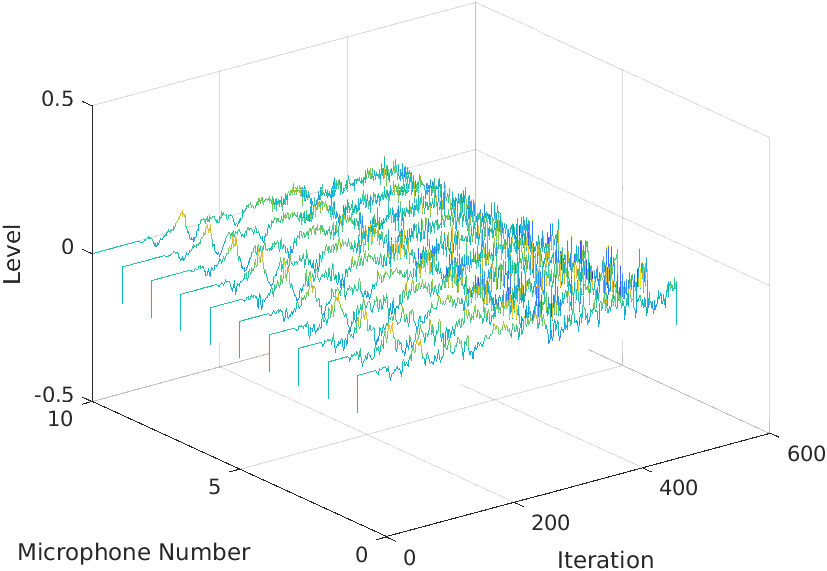
\includegraphics[width=75mm]{./Images/3_3_noise_noise_screen_3D.png}
        \caption{with screen}
        \label{fig_3_3_screen}
    \end{subfigure}
    \begin{subfigure}[]{75mm}
        \centering
        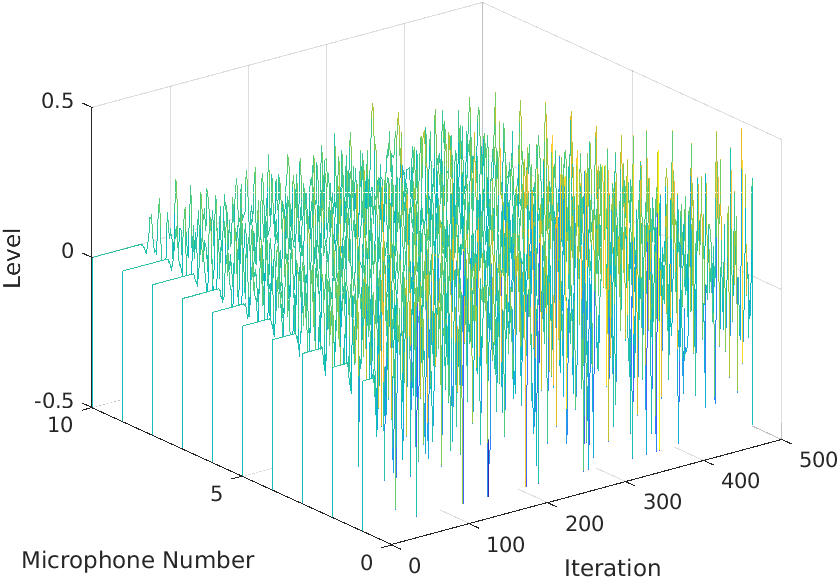
\includegraphics[width=75mm]{./Images/3_3_noise_no_screen_3D.png}
        \caption{without screen}
        \label{fig_3_3_no_screen}
    \end{subfigure}
    \caption{Example of signals received at the microphone array with and without noise screen using a noise source}
    \label{fig_3_3_3d}
\end{figure}

The calculation for the insertion loss was performed for all the variation of
sound sources and can be seen in Fig. \ref{fig_3_3_loss}.
One can observe that the noise screen generally provides a sound reduction.
It is the least effective for low frequency sine waves (NCPW $= 45$).
And the effectiveness seems to decrease over distance.

\begin{figure}[H]
    \centering
    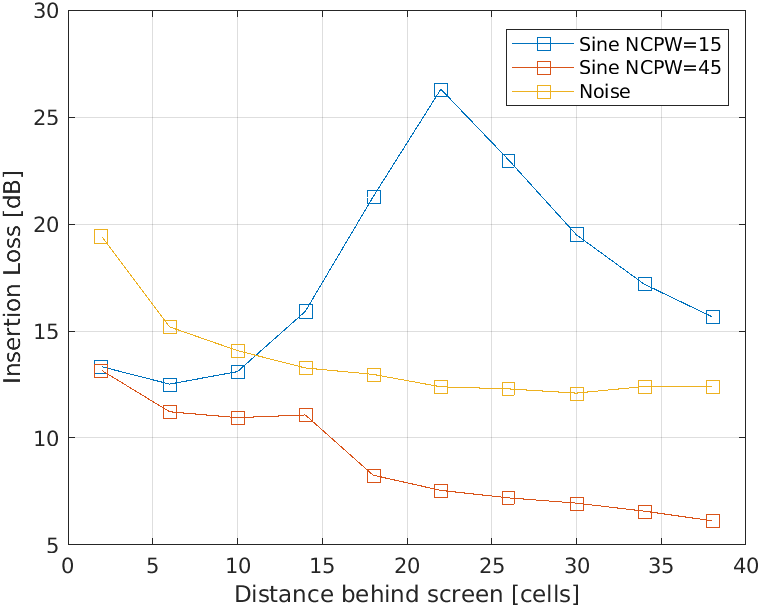
\includegraphics[width=75mm]{./Images/3_3_insertion_loss.png}
    \caption{Insertion loss for varying source types resulting from introducing a noise screen}
    \label{fig_3_3_loss}
\end{figure}

In the case of NCPW $= 15$ however, we can clearly see that, a strong attenuation takes
place at a certain distance after the screen.
This strong attenuation can be explained with an interference pattern that is
generated after the screen, which is displayed in Fig. \ref{fig_3_3_interference}.
We can see that with high frequency (NCPW $=15$) there's a beam of a local minimum that will
cross the height of the microphone array, resulting in the strong attenuation
that's seen in Fig. \ref{fig_3_3_loss}.

\begin{figure}[H]
    \begin{subfigure}[]{75mm}
        \centering
        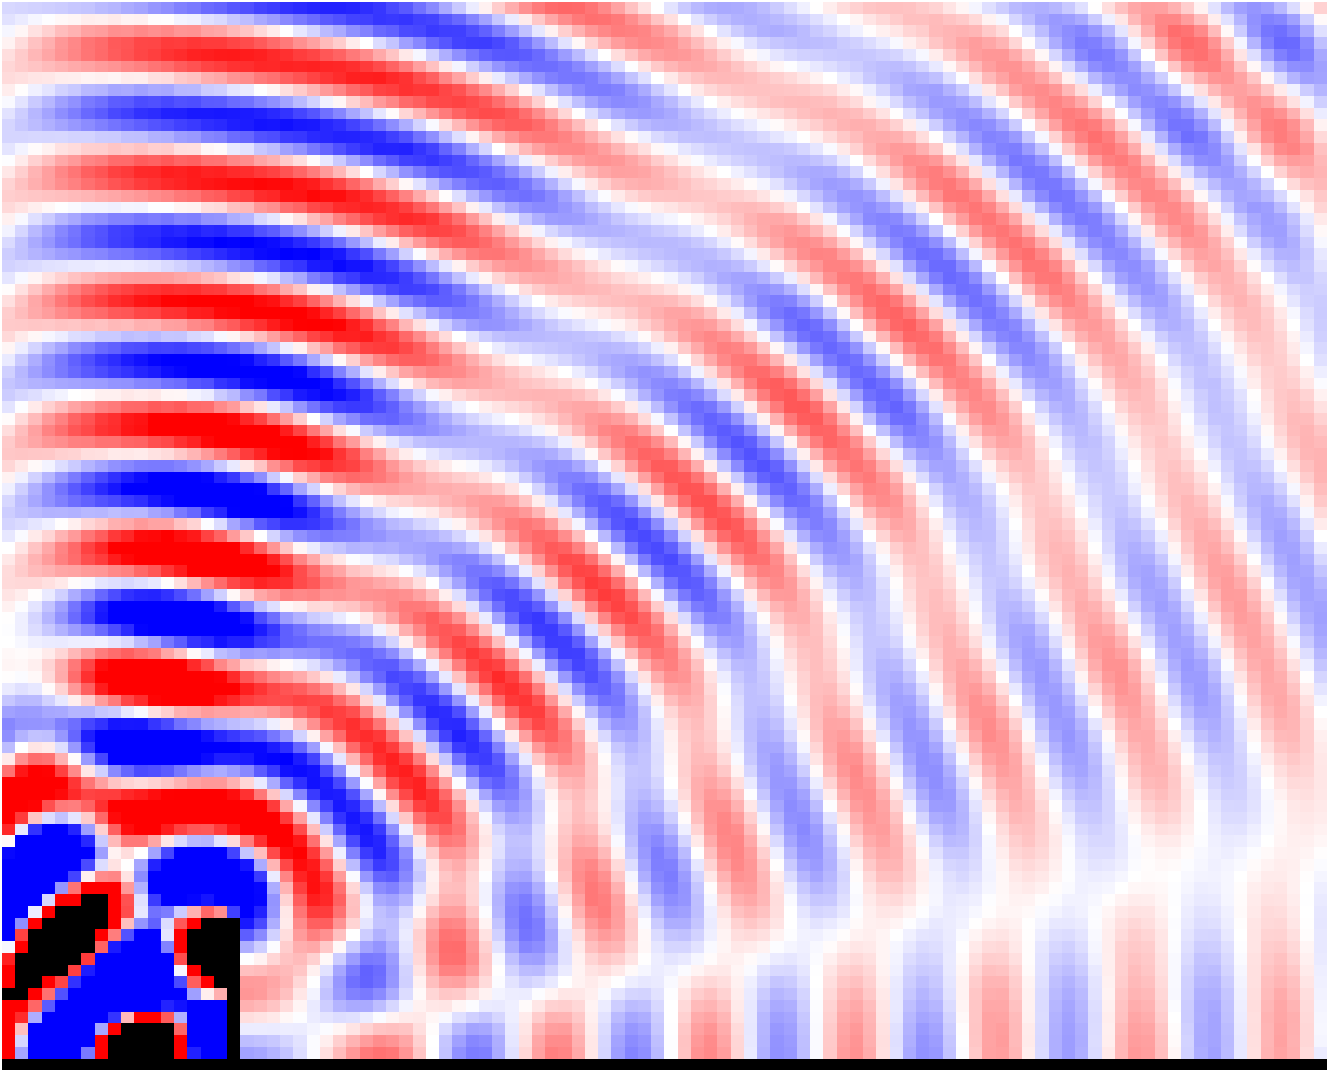
\includegraphics[width=50mm]{./Images/3_3_ncpw_15.png}
        \caption{NCPW $= 15$}
    \end{subfigure}
    \begin{subfigure}[]{75mm}
        \centering
        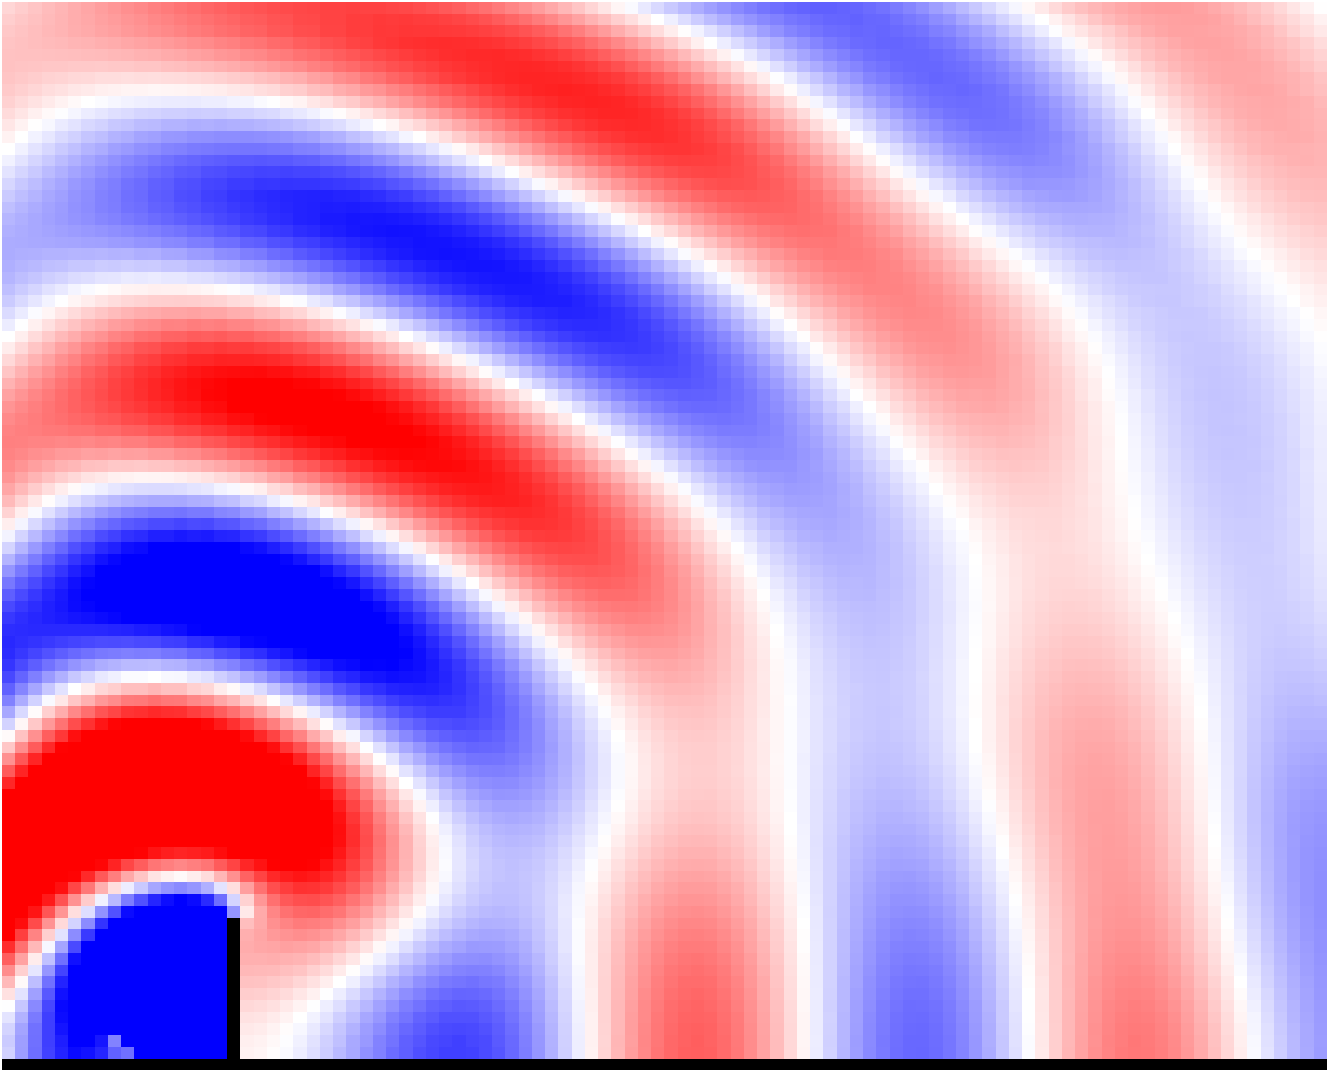
\includegraphics[width=50mm]{./Images/3_3_ncpw_45.png}
        \caption{NCPW $= 45$}
    \end{subfigure}
    \caption{Interference pattern after the noise screen for the two NCPW settings}
    \label{fig_3_3_interference}
\end{figure}

\section{Discussion}

\subsection{Python}
\subsubsection{Implementation}
The current implementation still seems somewhat faulty, when comparing the results
with TLMfig.
Debugging faults in the implementation took up more time than expected.
Due to that and not being able to completely fix all issues with the code, the frequency
response has not been implemeted yet.
And is therefore missing in the report.

\subsubsection{Matplotlib}
Using this library to plot the animation had some pitfalls.
The library uses a drawing buffer, which just fills over time.
Without manually clearing it before updating the plot, it will slow
the animation by a large amount.
Once that was introduced, a significant improvement could be observed.

\subsection{TLMfig}
While using this GUI some shortcomings were discovered.
Given that this might only be the case for the author's setup, which consisted
of a Linux machine without a dedicated GPU.

\subsubsection{Placing Objects}
Firstly, there are no coordinates for the cursor while drawing.
If this was the case placing objects in the plane would be simplified a lot.
A workaround is drawing lines as helpers and erasing them to all but one pixel
at the edge of the plane.
Nevertheless, this is only a minor issue.

\subsubsection{Exporting received signals}
Secondly, exporting the received data is not straightforward and this has some
overlap with the third observation.
Nevertheless possibilites could be to export the data which is plotted into the
Matlab workspace or generate a .mat file.
There's the option to export the configuration and grabbing the data from there,
but that's not exactly a logical step.

\subsubsection{Reusing stored configurations}
With talking about exporting the configuration we come to the third observation.
So assuming a configuration was saved and we reopen TLMfig.
Then try to open the stored configuration, it will open in a new TLMfig window.
This new window is solely a Matlab figure without the backend logic.
Therefore it cannot be used to re-run the stored configuration, making it impossible
to reproduce results without re-drawing the setup.

\subsubsection{GUI usage}
There are some additional unexpected behaviors.
E.g. the button label for placing mics updates to $1$ when a number is changed in the field,
then \textit{not} validated with the enter key, followed by clicking the button to place microphones.
It doesn't revert back and stays at the same number, which is $1$.

\begin{figure}[H]
    \centering
    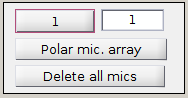
\includegraphics[width=35mm]{./Images/tlm_fig_button_label_bad.png}
    \caption{TLMfig button label after bug}
\end{figure}

Another unusual behavior is observed when using the input box to draw lines.
Sometimes one has to actually validate an input with the enter key and other times
it's enough to just change the value in the box and click somewhere else in the GUI
and a line is drawn.
This can lead to drawing way too many lines that were not intended if the user is not
aware of this.

\begin{figure}[H]
    \centering
    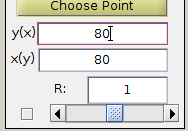
\includegraphics[width=35mm]{./Images/tlm_fig_updating_lines.png}
    \caption{Line drawing input box}
\end{figure}

\subsubsection{Conclusion}
All the observed issues are only hindering usability.
TLMfig otherwise seems to work as expected and the GUI is largely helpful
for simulating wave propagation and analzying propagation behavior in
various settings.


\section{References}

\small
\bibliographystyle{plain}
\bibliography{references}

\end{document}
